\section{Stable decisions}

Next step we need to do something more useful. And we reach the 'second form of a standard program', which means: A program that does something in it infinite loop.

This program stores one of two states and sets the LED on or off, keeping it according to the stored state. This explanation is slightly wrong. I try it again.

This program recognises an input signal consisting of two phases. A complete input signal consist of a LOW phase followed by a HIGH phase. The signal ends with entering the HIGH phase. We are interested only in change, as we always should.

If the Input signal changes from HIGH to LOW, our program changes the LED from its current state to the other state. If the LED was ON it will be set to OFF and vice versa. The state is only changed as reaction of changing the Input state from HIGH to LOW because 'no action' at the Input device leads to HIGH state in the input register as the result of using an internal 'pull up resistor' who does what he is called - he pulls the input signal up - to HIGH.

The electrical signal we are waiting for with our micro controller on our input pin is: Pulling it down to LOW (GND). And finally this is the Code to do it:

\begin{lstlisting}
.DEVICE atmega8

.org 0x0000
            rjmp    start

start:
            sbi     DDRB,         5
            cbi     DDRB,         4
            sbi     PORTB,        4

            ldi     r16,          1

main:
            sbic    PINB,         4
            rjmp    led_keep
            tst     r16
            breq    led_ok
            clr     r16
            sbis    PINB,         5
            rjmp    led_on
            cbi     PORTB,        5
            rjmp    led_ok
led_on:
            sbi     PORTB,        5
            rjmp    led_ok
led_keep:
            ldi     r16,          1
led_ok:
            rjmp    main
\end{lstlisting}


As you can see, this Code is not easy to understand. To do better, we add symbolic names to the soup. The basics are easy:

\begin{itemize}
  \item \texttt{.equ} means: 'a name for a number'
  \item \texttt{.def} means: 'a name for an entity'
\end{itemize}

So for example \texttt{DDRB} alread is a number. This number is defined in an include file chosen by you device selection. But in our case, whatever number is hidden behind the name DDRB it will be our Input/Output control port. So die name it \texttt{ctl} as prefix for 'control' and \texttt{IO} as name for Input\&Output.

In another example \texttt{bit} stands for 'bit number' and \texttt{Input} for 'Input bit' which makes \texttt{bitInput}, the bit where we red the input state.

You may define you own naming convention which should hold throughout your project.

\begin{lstlisting}
.DEVICE atmega8

.equ ctlIO     = DDRB    ; DDRB  is our I/O control register
.equ prtIO     = PORTB   ; PORTB is our I/O output port register
.equ pinIO     = PINB    ; PINB  is our I/O input pin register

.equ bitOutput = 5       ; pin 5 is our output bit
.equ bitInput  = 4       ; pin 4 is our input bit

.equ FALSE     = 0       ; 0 will be FALSE or OFF
.equ TRUE      = 1       ; 1 will be TRUE  or ON

.def bStatus   = r16     ; the last state will be stored in 'r16'
\end{lstlisting}

As you may not have expected, this makes the soup - or code - somehow better readable and so much easier to understand. Now it looks more like a higher language:

\begin{lstlisting}
.org 0x0000
            rjmp    start

start:
            sbi     ctlIO,        bitOutput
            cbi     ctlIO,        bitInput
            sbi     prtIO,        bitInput

            ldi     bStatus,      HIGH

main:
            sbic    pinIO,        bitInput
            rjmp    led_keep
            tst     bStatus
            breq    led_ok
            clr     bStatus
            sbis    pinIO,        bitOutput
            rjmp    led_on
            cbi     prtIO,        bitOutput
            rjmp    led_ok
led_on:
            sbi     prtIO,        bitOutput
            rjmp    led_ok
led_keep:
            ldi     bStatus,      HIGH
led_ok:
            rjmp    main
\end{lstlisting}

Even if it's a better reading, it seems no really to be easy to follow the program flow. So at first, we should introduce a program flow chart. And for good measure two of the. We need two of them to demonstrate a major point in assembler programming.

We have to take watch about WHAT we wish to do, but equally too about HOW we are going to do it.

\subsection{WHAT to do}

\begin{itemize}
  \item Initialise system and devices
  \item Wait for the change "input pin was HIGH and became LOW"
  \item Invert LED status
  \item Restart at (2)
\end{itemize}


\subsection{HOW to do it}

To get an impression on how to it, at first, we take a look at a flow diagram. This diagram shows the program flow outside the 'invert LED status' part. Changing the LED status currently is out of our focus. It is the very thing we try to deal with, but it is the more easy part of the solution.

\begin{figure}[htbp]
  \centering
  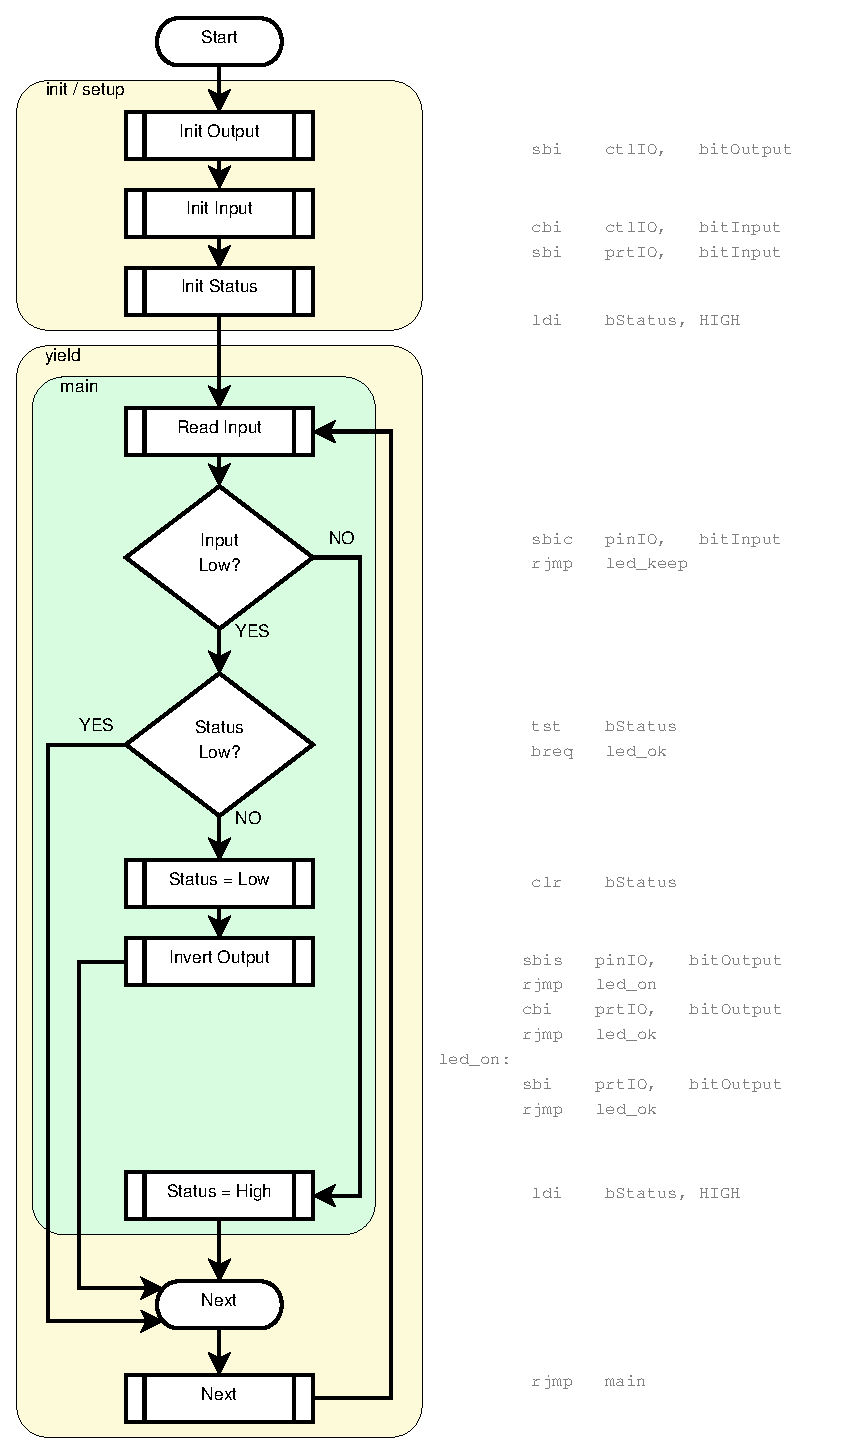
\includegraphics[height=210mm]{LED/S005_stable-decisions+symbols.eps}
  \caption{Stable Decisions Flow Diagram}
  \label{S005FlowDiagam}
\end{figure}

As you may found out until now, dealing with the 'human device interface' is the most complicated thing in informatics. It starts by the unbearable slowness of humans and does not end with humans expectations against machines.

At the moment out project restricts the 'human device problem' the unbearable slowness of humans.

A living entity presses a button and our device has to react. Our device may ask the input pin about 1.000.000 times per second. A human for example may to a short pressing of the button in about 0.2 seconds. Which means, our System reads the state 'button pressed' about 500.000 times during our humans action. But what the human expects is:

"Change the LED status ones as I press (in my view) the button ones!"

A second problem we will not deal with in this phase of our development is, that electric switches may flicker during status change.

So we simply have to ensure, that changing the LEDs status only happens ones per button press action. There are only two moments in all this endless button down phase where it is suitable to really change the LEDs status. At the beginning, as the signal changes from HIGH to LOW or at the end, where the signal changes from LOW to HIGH again.

To give the human who uses our device immediate feedback about success or failure of his action, we decide to use the first phase to do all the action. So we have a simple mission: If the signal is LOW now and was HIGH the last time we looked, we change the LEDs state. This satisfies also the endless LOW state of the input signal and the change from LOW to HIGH where we have to do nothing. Not even accidentally! This way, the human feels his request immediately answered, even if he is unable to comprehend how immediately it real is answered.

